\documentclass{article}\usepackage[]{graphicx}\usepackage[]{xcolor}
% maxwidth is the original width if it is less than linewidth
% otherwise use linewidth (to make sure the graphics do not exceed the margin)
\makeatletter
\def\maxwidth{ %
  \ifdim\Gin@nat@width>\linewidth
    \linewidth
  \else
    \Gin@nat@width
  \fi
}
\makeatother

\definecolor{fgcolor}{rgb}{0.345, 0.345, 0.345}
\newcommand{\hlnum}[1]{\textcolor[rgb]{0.686,0.059,0.569}{#1}}%
\newcommand{\hlsng}[1]{\textcolor[rgb]{0.192,0.494,0.8}{#1}}%
\newcommand{\hlcom}[1]{\textcolor[rgb]{0.678,0.584,0.686}{\textit{#1}}}%
\newcommand{\hlopt}[1]{\textcolor[rgb]{0,0,0}{#1}}%
\newcommand{\hldef}[1]{\textcolor[rgb]{0.345,0.345,0.345}{#1}}%
\newcommand{\hlkwa}[1]{\textcolor[rgb]{0.161,0.373,0.58}{\textbf{#1}}}%
\newcommand{\hlkwb}[1]{\textcolor[rgb]{0.69,0.353,0.396}{#1}}%
\newcommand{\hlkwc}[1]{\textcolor[rgb]{0.333,0.667,0.333}{#1}}%
\newcommand{\hlkwd}[1]{\textcolor[rgb]{0.737,0.353,0.396}{\textbf{#1}}}%
\let\hlipl\hlkwb

\usepackage{framed}
\makeatletter
\newenvironment{kframe}{%
 \def\at@end@of@kframe{}%
 \ifinner\ifhmode%
  \def\at@end@of@kframe{\end{minipage}}%
  \begin{minipage}{\columnwidth}%
 \fi\fi%
 \def\FrameCommand##1{\hskip\@totalleftmargin \hskip-\fboxsep
 \colorbox{shadecolor}{##1}\hskip-\fboxsep
     % There is no \\@totalrightmargin, so:
     \hskip-\linewidth \hskip-\@totalleftmargin \hskip\columnwidth}%
 \MakeFramed {\advance\hsize-\width
   \@totalleftmargin\z@ \linewidth\hsize
   \@setminipage}}%
 {\par\unskip\endMakeFramed%
 \at@end@of@kframe}
\makeatother

\definecolor{shadecolor}{rgb}{.97, .97, .97}
\definecolor{messagecolor}{rgb}{0, 0, 0}
\definecolor{warningcolor}{rgb}{1, 0, 1}
\definecolor{errorcolor}{rgb}{1, 0, 0}
\newenvironment{knitrout}{}{} % an empty environment to be redefined in TeX

\usepackage{alltt}
\usepackage{amsmath} %This allows me to use the align functionality.
                     %If you find yourself trying to replicate
                     %something you found online, ensure you're
                     %loading the necessary packages!
\usepackage{amsfonts}%Math font
\usepackage{graphicx}%For including graphics
\usepackage{hyperref}%For Hyperlinks
\usepackage[shortlabels]{enumitem}% For enumerated lists with labels specified
                                  % We had to run tlmgr_install("enumitem") in R
\hypersetup{colorlinks = true,citecolor=black} %set citations to have black (not green) color
\usepackage{natbib}        %For the bibliography
\setlength{\bibsep}{0pt plus 0.3ex}
\bibliographystyle{apalike}%For the bibliography
\usepackage[margin=0.50in]{geometry}
\usepackage{float}
\usepackage{multicol}

%fix for figures
\usepackage{caption}
\newenvironment{Figure}
  {\par\medskip\noindent\minipage{\linewidth}}
  {\endminipage\par\medskip}
\IfFileExists{upquote.sty}{\usepackage{upquote}}{}
\begin{document}

\vspace{-1in}
\title{Lab 3 -- MATH 240 -- Computational Statistics}

\author{
  Pierce Leclerc \\
  Colgate University  \\
  Department of Mathematics  \\
  {\tt pleclerc@colgate.edu}
}

\date{}

\maketitle

\begin{multicols}{2}
\begin{abstract}

Musical data from The Front Bottoms, Manchester Orchestra, and All Get Out was collected, cleaned, and merged with lyrical data. Data from the collaborative track ``Allentown" was isolated to determine which artist was most closely aligned with its production and sound. Box plots of musical and lyrical parameters suggest that ``Allentown" aligns closest with Manchester Orchestra, with statistical analysis suggesting a similar conclusion.
\end{abstract}

\noindent \textbf{Keywords:} Music Analysis, Batch Files, Data Compilation, Data Cleaning

\section{Introduction}

In 2018, The Front Bottoms, Manchester Orchestra, and All Get Out collaborated on a song entitled ``Allentown". Our goal in this project is to determine which band contributed more to the song by analyzing the music from both bands and comparing data from the new song to their respective collections. In Lab 2, we set up the code for processing each individual track, building a batch file containing the specific lines of code for each song that we can run to collect data using executable files of Essentia \citep{essentia}. In Lab 3, we compiled data from Essentia and combined the musical data with lyrical data into one data frame. Parameters were plotted using box plots to compare data between each artist and the track ``Allentown". In Lab 5, a function was created to determine whether a given numerical descriptor for ``Allentown" was in range, outlying, or out of range of the descriptors from each individual artist's songs.

\section{Methods}

In Lab 2, we began by utilizing tools from the \texttt{stringr} package for \texttt{R} to collect the names of tracks, albums, and artists \citep{str}. We combined them to create unique names for each track's output \texttt{.json} file. We then utilized the \texttt{writeLines()} function to write a line of code specific to each track into a batch file. Lastly, we took the sample song Au Revoir (Adios) by The Front Bottoms and analyzed specific characteristics of the song with the \texttt{jsonlite} package for \texttt{R} \citep{jsl}.

\subsection{Compiling and Cleaning Essentia Data}

In Lab 3, we took each \texttt{.json} file and extracted musical data from each track. From the Essentia models, we then extracted musical characteristics of each song, including overall loudness, spectral energy, dissonance, pitch salience, tempo (BPM), beat loudness, danceability, and tuning frequency. We compiled the data from all the songs into a data frame, and included additional data from the Essentia models. \texttt{valence}, \texttt{arousal}, and \texttt{timbre} were included, alongside moods such as \texttt{aggressive}, \texttt{happy}, \texttt{party}, \texttt{relaxed}, and \texttt{sad}. Sound characteristics like \texttt{acoustic}, \texttt{electric}, and \texttt{instrumental} were accounted for as well. Lyrical data from the text analysis tool LIWC was subsequently analyzed and merged into the existing data frame. 

\section{Results}

Once the data frame was assembled, two \texttt{.csv} files were created to separate ``Allentown" from the rest of the songs. Sound and lyrical value of the songs from each artist were grouped in box plots and compared to the spectral energy and linguistic value from ``Allentown".

\subsection{Box Plots: Spectral Energy, Linguistic Value}

\begin{center}
  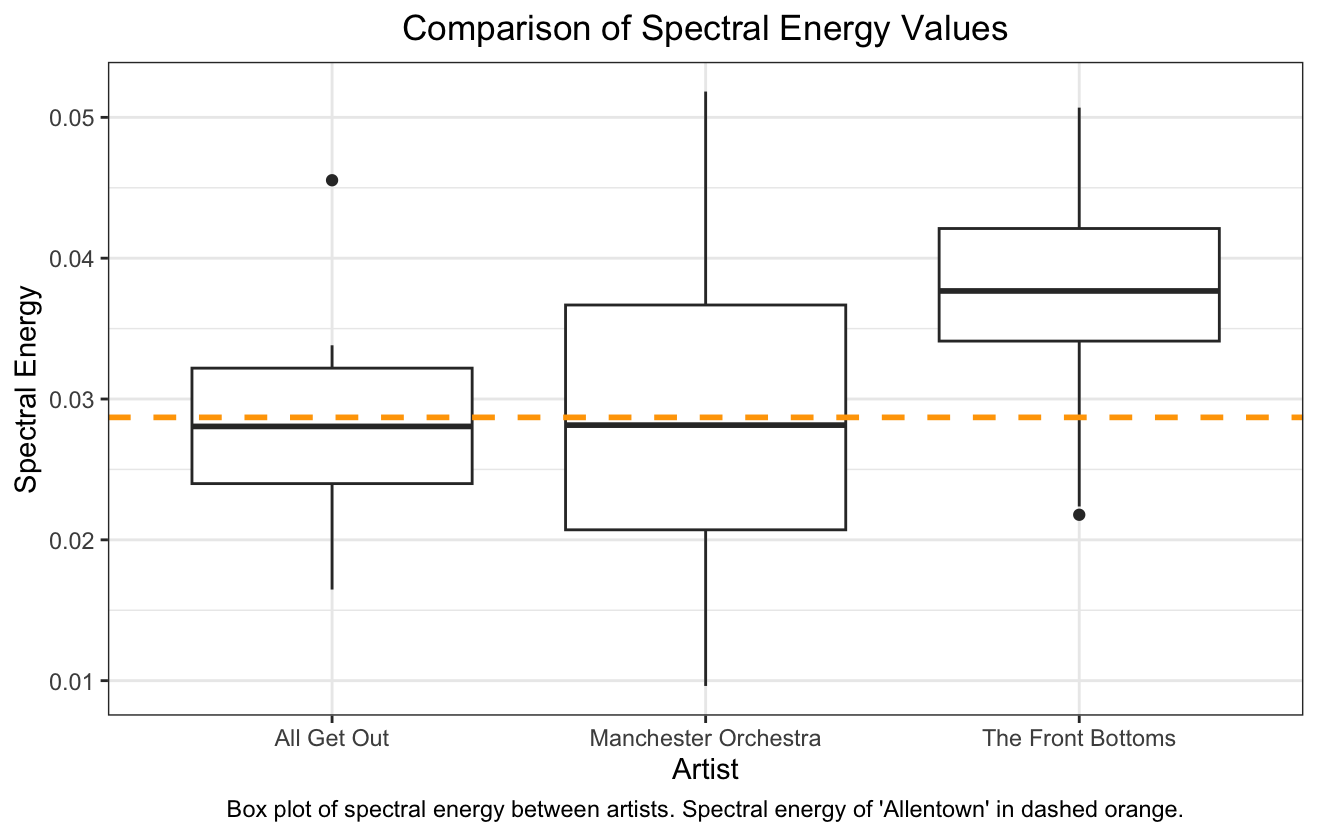
\includegraphics[width=0.5\textwidth]{boxplot_se.png}
  \newpage
  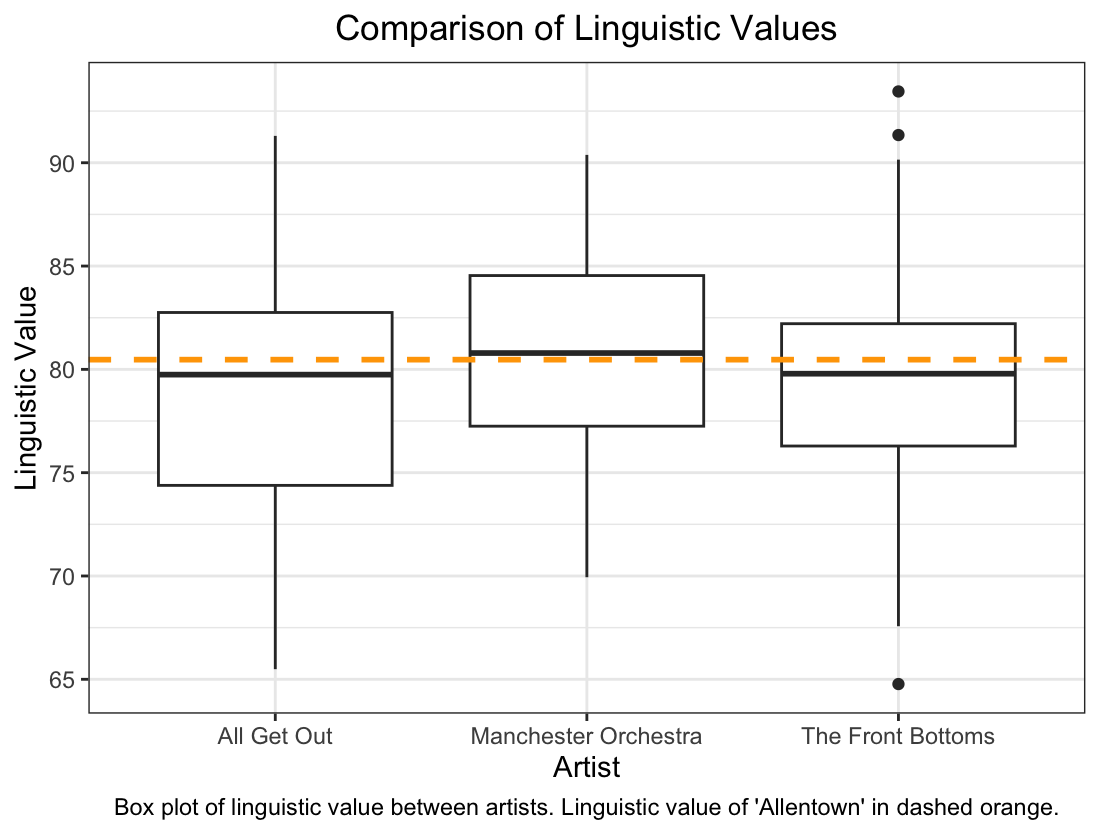
\includegraphics[width=0.5\textwidth]{boxplot_linguistic.png}
\end{center} 

In Lab 5, a table was created to store the quantities of each descriptor status by artist. It is clear numerically that Manchester Orchestra has the lowest number of descriptors that are out of range from ``Allentown" and the largest number of descriptors in range.

\begin{table}[H]
\centering
\scriptsize
\begin{tabular}{rlrrr}
  \hline
 & Artist & Out of Range & Outlying & Within Range \\ 
  \hline
1 & All Get Out &  22 &  17 & 158 \\ 
  2 & Manchester Orchestra &   3 &  11 & 183 \\ 
  3 & The Front Bottoms &  30 &  11 & 156 \\ 
   \hline
\end{tabular}
\caption{Count of descriptor status for "Allentown" between artists.} 
\label{tab:reference}
\end{table}

A bar graph was also created to visualize the data from the above table.

\begin{center}
  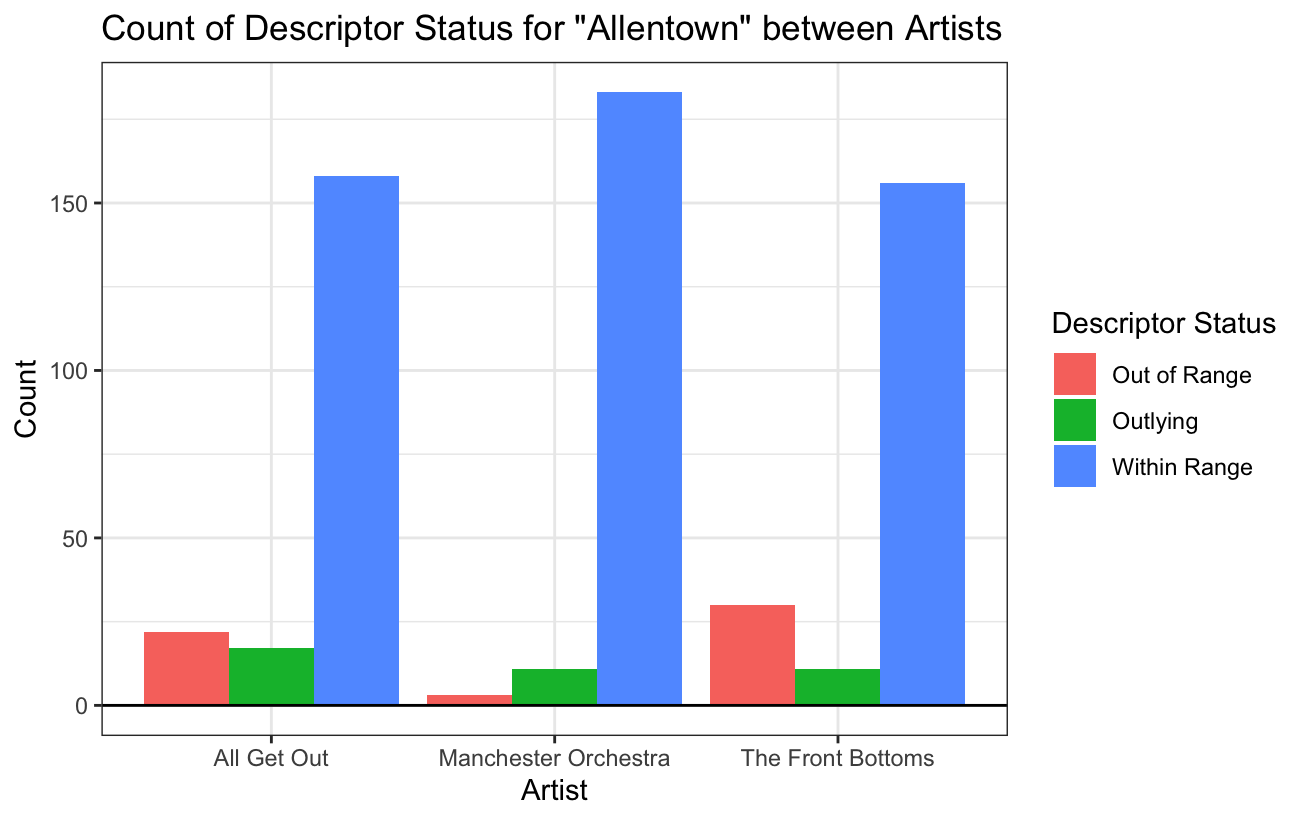
\includegraphics[width=0.5\textwidth]{descriptors.png}
\end{center} 

\section{Discussion}

From the spectral energy box plot, it is evident that ``Allentown" is much more closely aligned to the medians of All Get Out and Manchester Orchestra, while distant from The Front Bottoms. Lyrically, the box plot of linguistic value indicates relation to all three artists, although most closely aligned to the median of Manchester Orchestra once again. \\

\noindent In evaluation of both musical and lyrical characteristics, it appears that ``Allentown" is more closely related to Manchester Orchestra than The Front Bottoms. By grouping the descriptors by artist, and comparing their summary values to the descriptor values of ``Allentown," it is evident that Manchester Orchestra has the closest alignment overall, as only 3 of the 197 descriptors are out of range.

%%%%%%%%%%%%%%%%%%%%%%%%%%%%%%%%%%%%%%%%%%%%%%%%%%%%%%%%%%%%%%%%%%%%%%%%%%%%%%%%
% Bibliography
%%%%%%%%%%%%%%%%%%%%%%%%%%%%%%%%%%%%%%%%%%%%%%%%%%%%%%%%%%%%%%%%%%%%%%%%%%%%%%%%
\vspace{2em}

\begin{tiny}
\bibliography{bib}
\end{tiny}
\end{multicols}

%%%%%%%%%%%%%%%%%%%%%%%%%%%%%%%%%%%%%%%%%%%%%%%%%%%%%%%%%%%%%%%%%%%%%%%%%%%%%%%%
% Appendix
%%%%%%%%%%%%%%%%%%%%%%%%%%%%%%%%%%%%%%%%%%%%%%%%%%%%%%%%%%%%%%%%%%%%%%%%%%%%%%%%
\newpage
\onecolumn

\end{document}
